% a tikz figure for audio processing pipeline

\usetikzlibrary{shapes}

\tikzstyle{data}=[draw,thick,rounded corners,minimum height=1.5cm,text width=2cm,align=center]
\tikzstyle{process}=[rectangle,draw,thick,minimum height=1.5cm,text width=2cm,align=center]

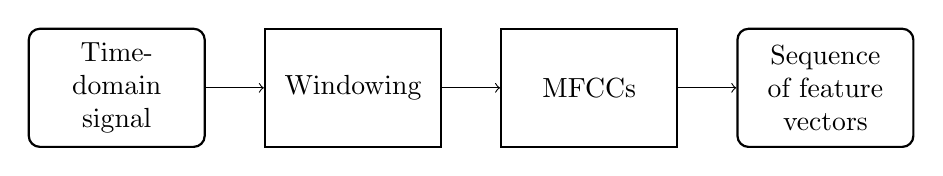
\begin{tikzpicture}[]
  \node[data] (i) at (0,0) {Time-domain signal};
  \node[process] (p1) at (3,0) {Windowing}
    edge [<-] (i);
  \node[process] (p2) at (6,0) {MFCCs}
    edge [<-] (p1);
  \node[data] (o) at (9,0) {Sequence of feature vectors}
    edge [<-] (p2);
\end{tikzpicture}

